\subsection*{Model}
The function described in this problem is the following 
\begin{equation*}
\begin{aligned}
    &F(\boldsymbol{x}) = \frac{1}{2}\sum_{k=1}^n f_k^2(\boldsymbol{x}) \\
    &f_k(\boldsymbol{x}) = x_k-1, & k=1 \\
    &f_k(\boldsymbol{x}) = 10(k-1)(x_k - x_{k-1})^2, & 1<k\leq n
\end{aligned}
\end{equation*}
where $n$ is the length of the input vector $\boldsymbol{x}$.
With the given starting point for minimization being 
\[\boldsymbol{x_0}=[-1.2,-1.2,...,-1.2,-1]' \in \mathbbm{R}^n.\]
The gradient of $F(\boldsymbol{x})$ is the following (note that, besides the first and last components, all the others have the same structure).
\begin{equation*}
    \nabla F(\mathbf{x}) = 
    \begin{bmatrix}
        \frac{\partial F}{\partial x_1}(\mathbf{\boldsymbol{x}}) \\
        \vdots \\
        \frac{\partial F}{\partial x_k}(\mathbf{\boldsymbol{x}}) \\
        \vdots \\
        \frac{\partial F}{\partial x_n}(\mathbf{\boldsymbol{x}})
    \end{bmatrix}
    =
    \begin{bmatrix}
        \frac{\partial }{\partial x_1}\frac{1}{2}(f_1^2+f_2^2)(\boldsymbol{x}) \\
        \vdots \\
        \frac{\partial F}{\partial x_k}\frac{1}{2}(f_k^2+f_{k+1}^2)(\boldsymbol{x}) \\
        \vdots \\
        \frac{\partial F}{\partial x_n}\frac{1}{2}f_n^2(\boldsymbol{x})
    \end{bmatrix}
    =
    \begin{bmatrix}
        x_1-1-200\cdot (x_2-x_1)^3 \\
        \vdots \\
        200 \cdot \Big((k-1)^2(x_k-x_{k-1})^3-k^2(x_{k+1}-x_k)^3\Big)\\
        \vdots \\
        200 \cdot (n-1)^2(x_n-x_{n-1})^3
    \end{bmatrix}
\end{equation*}
The Hessian matrix of $F(\boldsymbol{x})$ is sparse since only on three diagonals elements different from zeros are present. They are the following:
\begin{align*}
    \frac{\partial^2 F}{\partial x_1^2} (\boldsymbol{x}) &= 1+600\cdot(x_2-x_1)^2 \\
    \frac{\partial^2 F}{\partial x_k^2} (\boldsymbol{x}) &= 600\cdot\Big((k-1)^2(x_k-x_{k-1})^2+k^2(x_{k+1}-x_k)^2 \Big), \quad 1 < k < n  & \\
    \frac{\partial^2 F}{\partial x_n^2} (\boldsymbol{x}) &=600\cdot(n-1)^2(x_n-x_{n-1})^2 \\
    \frac{\partial^2 F}{\partial x_k \partial x_{k-1}} (\boldsymbol{x}) &= -600\cdot (k-1)^2(x_k-x_{k-1})^2, \quad 1<k\leq n.
\end{align*}
It is easy to notice that $F$, being the sum of squared functions, is always non negative. Furthermore, $F(\boldsymbol{x})=0$ if and only if $\boldsymbol{x}=[1,1,...,1]'$ since $f_1(\boldsymbol{x})^2=0$ if and only if $x_1=1$ and, for every $1<k\leq n$, $f_k(\boldsymbol{x})=0$ if and only if $x_k=x_{k-1}$.

More formally, we can see that $\boldsymbol{x}=[1,1,...,1]'$ solves the equation $\nabla F(\boldsymbol{x})=\boldsymbol{0}$. Since $F$ is convex (being the sum of convex functions) and differentiable, we know that any stationary point is a global minimum point for $F$. 

Then $\boldsymbol{x}=[1,1,...,1]'$ is the only global minimum point for $F$.

We plot the function for $n=2$ in a neighborhood of the minimum point.
\begin{figure}[H]
    \centering
    \begin{subfigure}{0.45\textwidth}
        \centering
        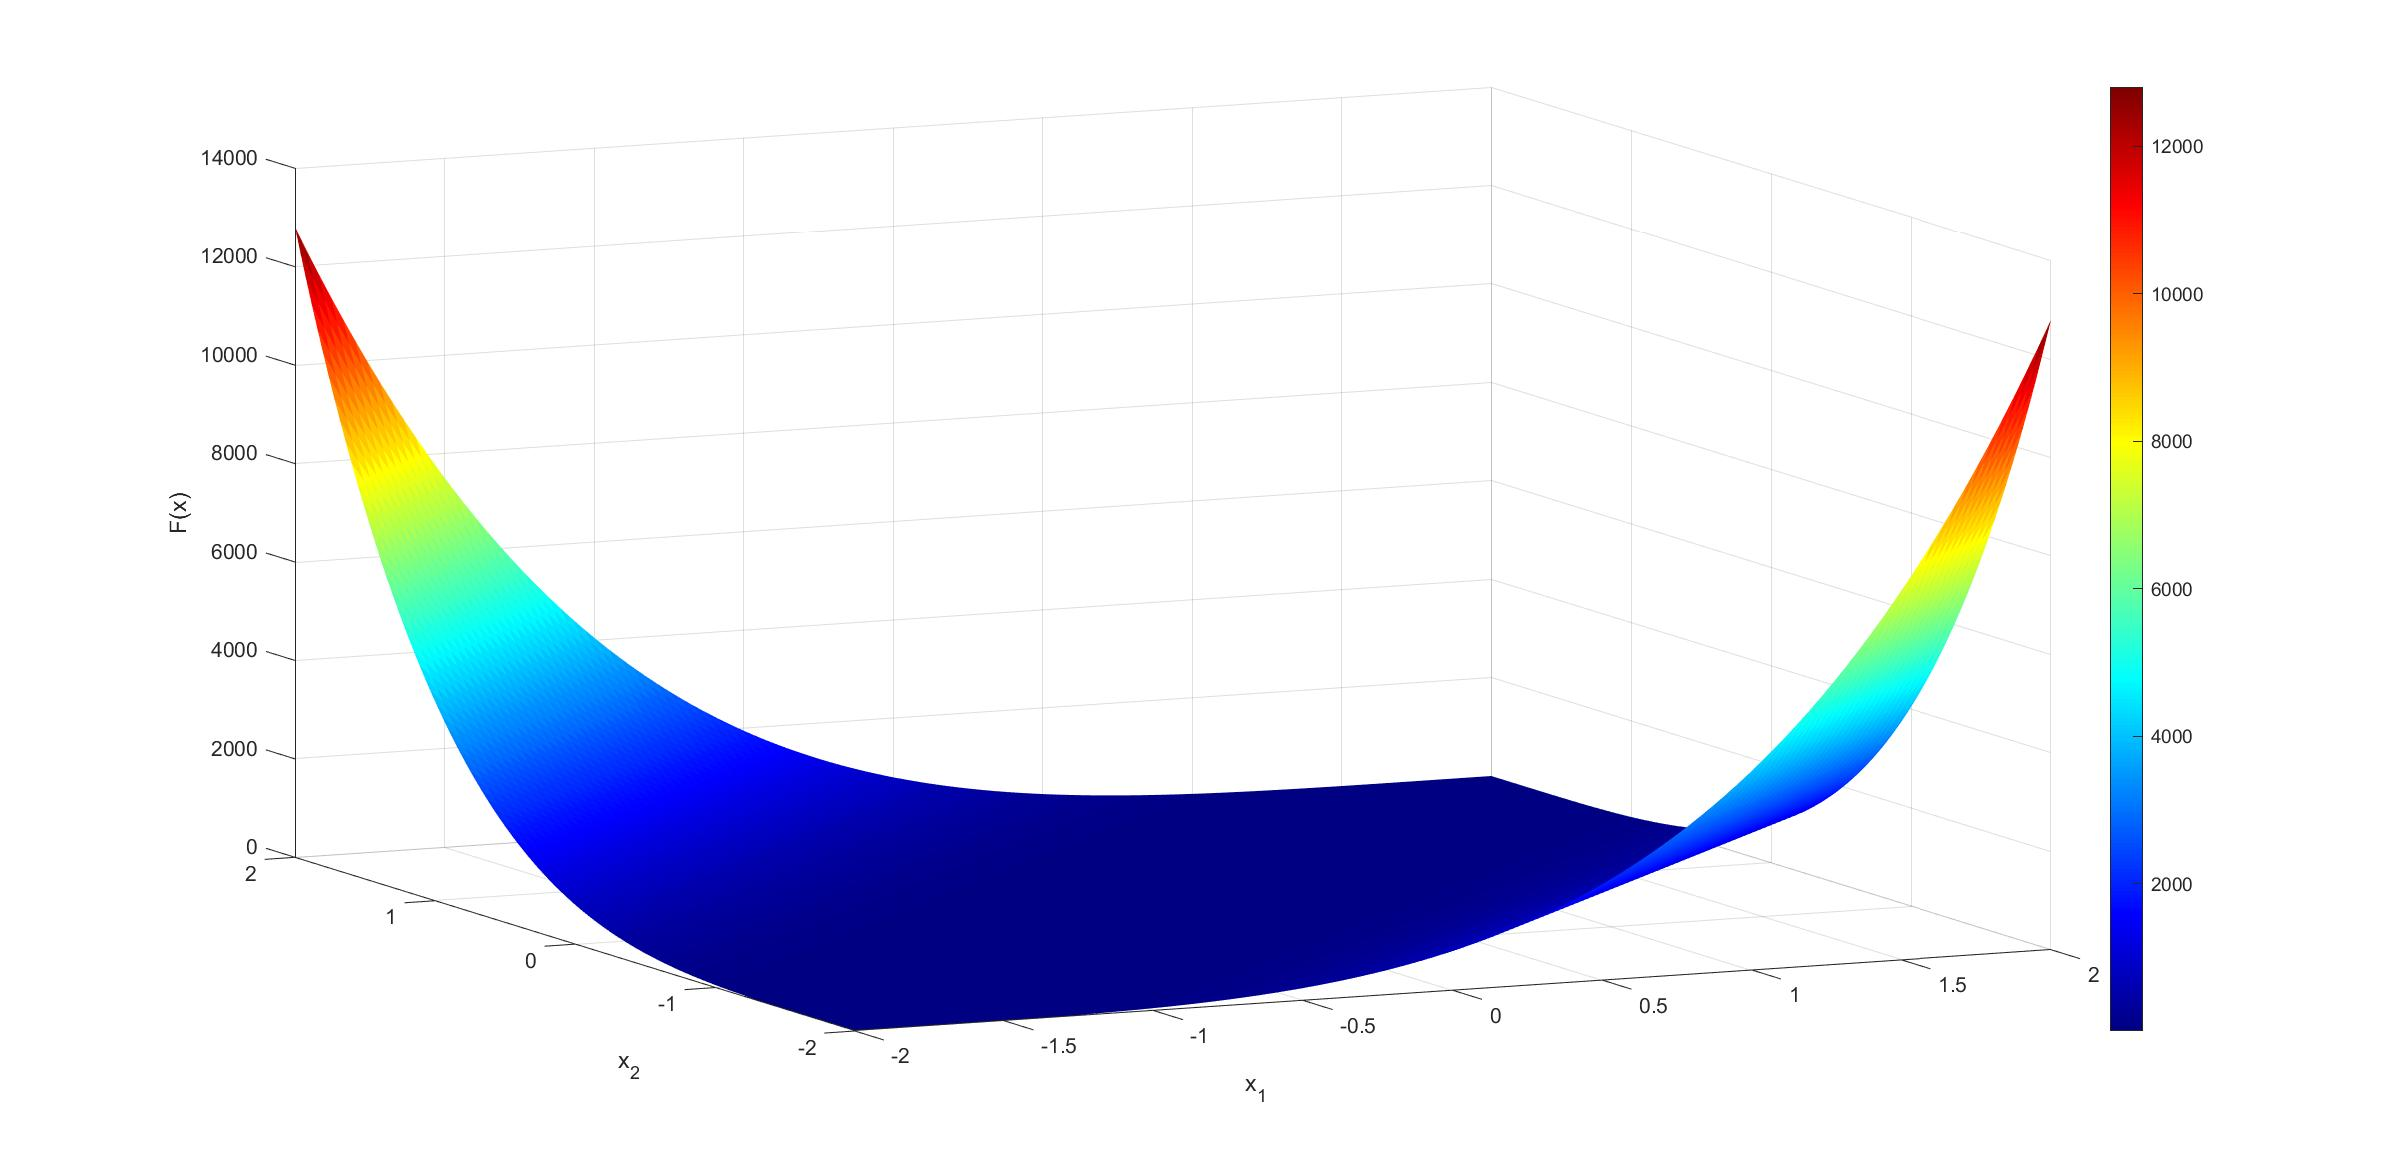
\includegraphics[width=\textwidth]{img/function_pb75_angolo1.jpg}
        \caption{}
    \end{subfigure}
    \begin{subfigure}{0.45\textwidth}
        \centering
        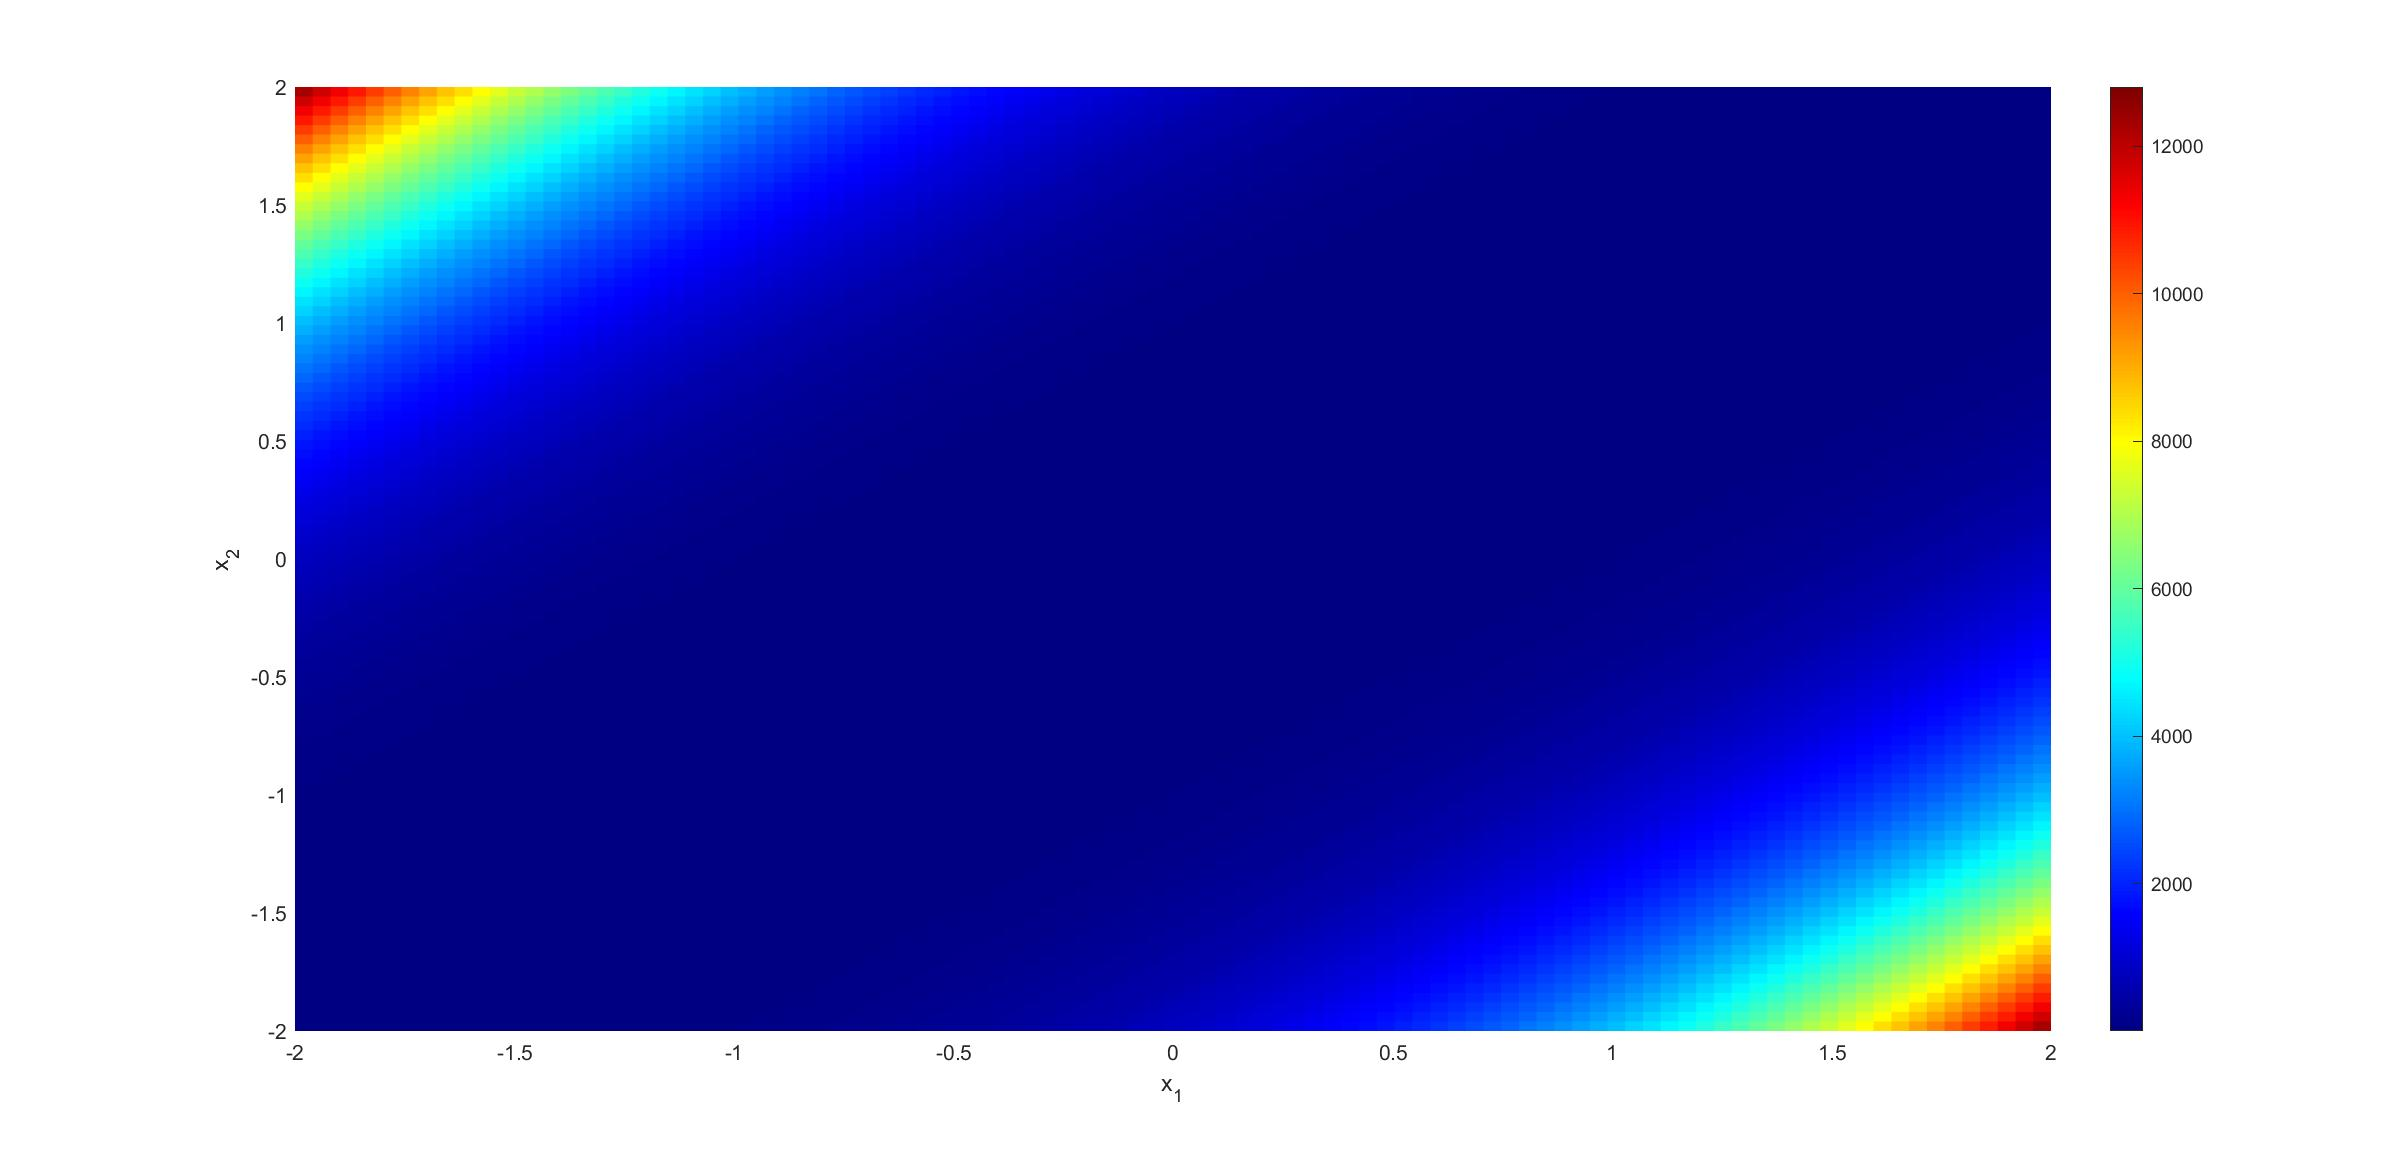
\includegraphics[width=\textwidth]{img/function_pb75_angolo2.jpg}
        \caption{}
    \end{subfigure}
    \caption{function $F(\boldsymbol{x})$ for $n=2$}
%\label{fig:funzione 2D pb 75}
\end{figure}
We can easily see that the central area, where the minimum point is located,
is quite flat. This means that the minimization methods used might have some troubles
when reaching this area because they might get stuck before reaching the minimizer.

\subsection*{Nelder Mead Method}
We runned the minimisation problem with Nelder Mead method using the following parameters:
\begin{eqnarray*}
    \text{reflection } \rho &=& 1.1 \\
    \text{expansion } \chi &=& 2.5 \\
    \text{contraction } \gamma &=& 0.6 \\
    \text{shrinking } \sigma &=& 0.5.
\end{eqnarray*}
The aim, with this choice, is to try to keep the simplex big enough so that
the method will not get stuck too easily in the almost flat areas of the function's graph.

We now report a table summarizing the results obtained by running the Nelder-Mead method
on the considered problem for dimensions $n=$10, 25, 50 and for a total of 11 starting 
points for each dimension, obtained as perturbations of the given one.

\begin{figure}[H]
    \centering
    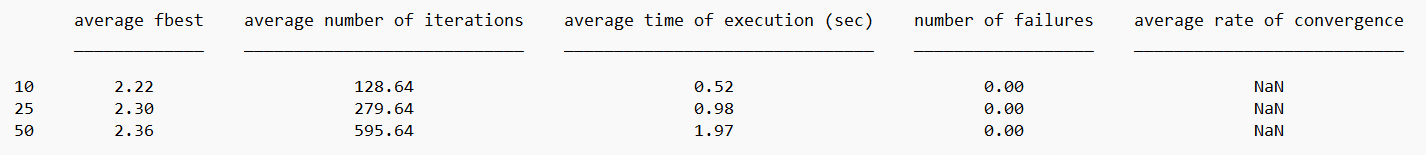
\includegraphics[width=1\textwidth]{img/pb75_table_SX.png}
    \caption{Results obtained by running the Nelder Mead method on problem 75.} 
    \label{pb 75 table SX}
\end{figure}

We notice that the method reports zero failures, which means that it never stopped because of the maximum 
number of iterations allowed (in this case $200\cdot n$) had been reached. However, the best value of the 
function $F$ that has been found is not so close to the expected value (which as observed before should be 0).
The problem is in the starting point. In fact, even with the random perturbations, it always falls in the flat area 
of the function. Tuning the parameters in a way that encourages the expansion of the simplex's area is not enough 
to prevent the method from getting stuck here. It can be seen that, if we use as a staring point for example $[0,0,...,0]'$, 
the results are a bit closer to the exact one (around 0.35). 

The Nelder Mead method does not guarantee convergence and it is sensitive to the starting point and this becomes evident 
in this optimisation problem.

Concerning the rate of convergence, the fact that \verb+Nan+ is always reported is due to the construction of the method
itself. In fact not necessarily at every iteration the best point of the current simplex is updated; expecially when contraction
and shrinking phases are reached, it means that new promising points were not found, so it is quite likely that the current best point
does not change among consecutive iterations. This is a problem when it comes to apply the formula for the experimental rate of 
convergence $\eqref{definizione_roc}$, since it leads the denominator to be 0.

\medskip
\subsection*{Modified Newton Method - Exact Derivatives}
As previously shown, we can easily compute the exact derivatives for the gradient and the Hessian matrix of $F(x)$. The Hessian should be stored
as a sparse matrix due to its large dimension. We can then apply the Modified Newton Method to the considered problem, obtaining the following 
results. 
\begin{figure}[H]
    \centering
    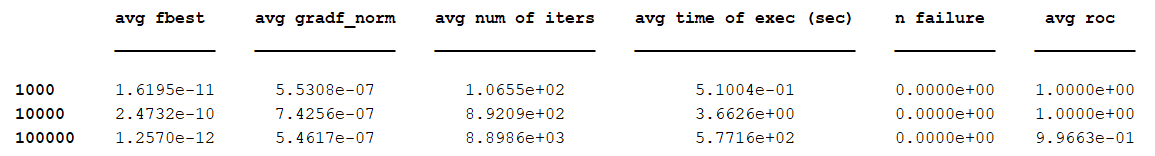
\includegraphics[width=1\textwidth]{img/pb75_table_MN.png}
    \caption{Results obtained by running the Modified Newton method on problem 75 using exact derivatives.} 
    \label{pb 75 table MN}
\end{figure}
As expected, this method is performing much better due to the exploitation of the information contained in the gradient and the Hessian. 
In every tested dimension $n$ it reaches the exact solution within the maximum number of iterations fixed for the corresponding dimension
(in this case $n$ has been used). For the others parameters the following values have been used:
\begin{itemize}
    \item tolerance for the norm of the gradient: $10^{-6}$ for every dimension
    \item parameter $\rho \in (0,1)$ for the reduction of the steplength in backtracking: $\rho$= 
    $\begin{cases}
        0.4 \quad n=10^3 \\
        0.3 \quad n=10^4 \\
        0.4 \quad n=10^5
    \end{cases}$
    \item parameter $c_1 \in (0,1)$ for the Armijo condition: $c_1$= 
    $\begin{cases}
        10^{-4} \quad n=10^3 \\
        10^{-4} \quad n=10^4 \\
        10^{-3} \quad n=10^5
    \end{cases}$
    \item maximum number of backtracking steps allowed: \texttt{btmax} = 
    $\begin{cases}
        36 \quad n=10^3 \\
        28 \quad n=10^4 \\
        36 \quad n=10^5
    \end{cases}$ 
\end{itemize}
The values of $\rho$ and \texttt{btmax} for every dimension has been chosen in such a way that stagnation is not allowed. 
In fact $\rho^{\texttt{btmax}}>\epsilon_m$, where the machine precision is $\epsilon_m \approx 10^{-16}$.

That experimental rate of convergence is approximately 1, so we are losing some of the strength of pure Newton method. 

In the following figure we can see two examples of the progress of the minimum value of $F(x)$.
\begin{figure}[htbp]
    \centering
    % Prima immagine
    \begin{subfigure}[t]{0.45\textwidth}  % Larghezza del 45% del testo
        \centering
        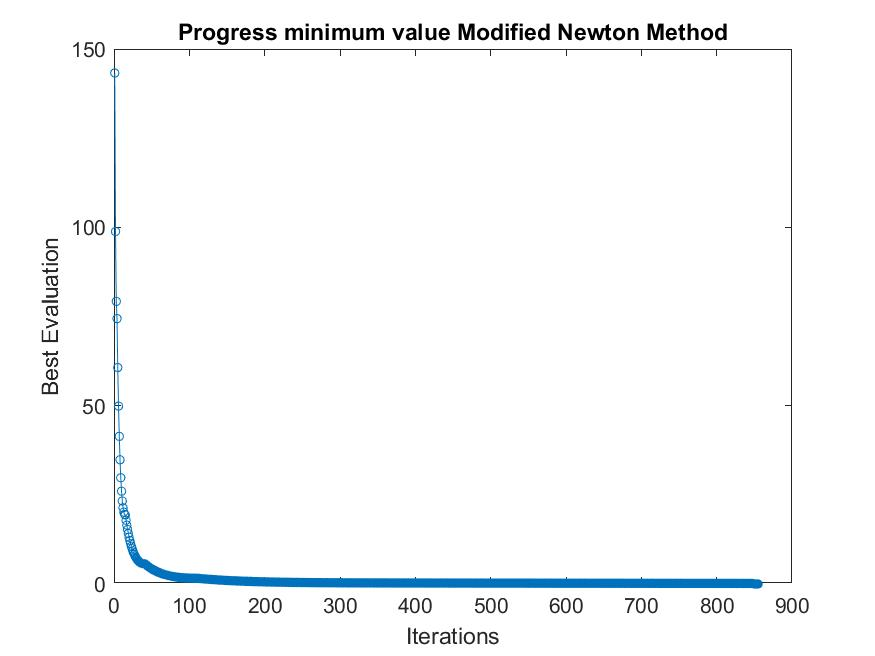
\includegraphics[width=\textwidth]{img/pb75_1e3_MN_convergence.jpg}
        \caption{$n=10^3$}
    \end{subfigure}
    \hspace{1cm} %spaziatura tra le immagini
    % Seconda immagine
    \begin{subfigure}[t]{0.45\textwidth}
        \centering
        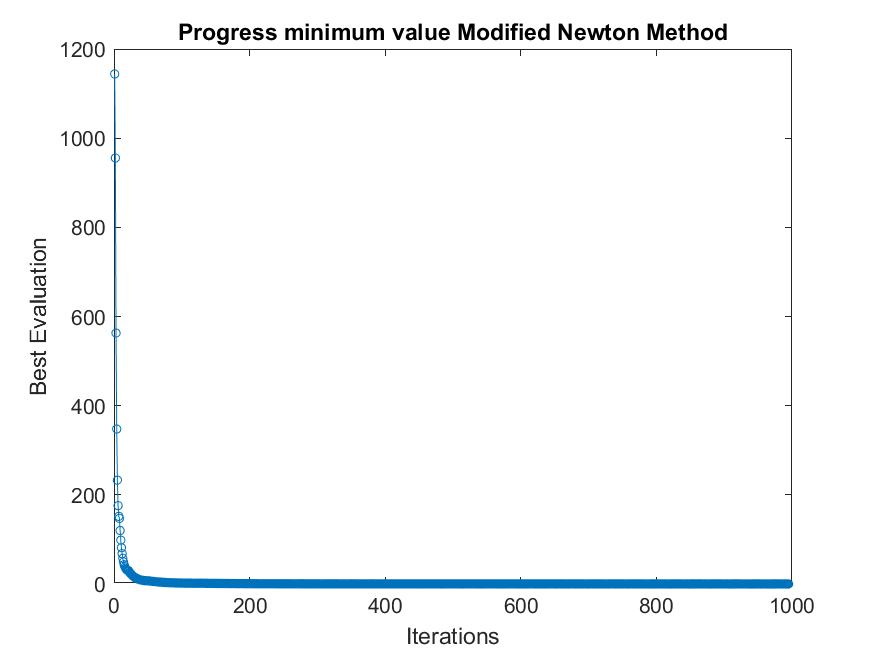
\includegraphics[width=\textwidth]{img/pb75_1e4_MN_convergence.jpg}
        \caption{$n=10^4$}
    \end{subfigure}
    % Didascalia generale
    \caption{Example of convergence to zero of the value of $F(x)$.}
    \label{convergenze MN 75}
\end{figure}
Notice how fast it decreases in the first iterations, while the convergence becomes smaller when entering the almost flat area of the function.

\medskip
\subsection*{Modified Newton Method - Approximated Derivatives}
Let us now analyze what happens if we suppose not to be able to compute the exact derivatives of function $F$.

Using forward difference with step $h_k$ (where $h_k$ can either be constant or $h_k=h|\hat{x}_k|$ where $k=1,...,n$ and $\hat{x}$ is the point 
where the approximation is calculated), we can obtain an approximation of the gradient of $F$. We denote as $\vec{e_k} \in \mathbbm{R}^n$ the k-th vector of the canonic basis. 
Note that we can exploit the structure of the function
in order to avoid the evaluation of the whole $F$. This makes the evaluation much faster.
\begin{eqnarray*}
    \frac{\partial F}{\partial x_k}(x) &\approx& \frac{F(x+h_k \vec{e_k})-F(x)}{h_k} 
    = \frac{f_k^2(x+h_k \vec{e_k}) +f_{k+1}^2(x+h_k\vec{e_k}) -f_k^2(x) -f_{k+1}^2(x) }{2h_k} \quad 1\leq k<n \\
    \frac{\partial F}{\partial x_n}(x) &\approx& \frac{f_n^2(x+h_n\vec{e_n}) - f_n^2(x)}{2h_n}.
\end{eqnarray*}
The same reasoning can be applied to approximate the Hessian using the general formula 
$$\frac{\partial^2 f}{\partial x_i \partial x_j} (x) \approx \frac{f(x+h_i\vec{e_i}+h_j\vec{e_j}) - f(x+h_i\vec{e_i}) - f(x+h_j\vec{e_j}) + f(x) }{h_ih_j}$$
and recalling that each $f_k$ for $1<k\leq n$ only depends on $x_k$ ad $x_{k-1}$. We obtain the following 
\begin{eqnarray*}
    \frac{\partial^2 F}{\partial x_k^2} &\approx& \frac{f_k^2(x+2h_k\vec{e_k}) + f_{k+1}^2(x+2h_k\vec{e_k}) -2f_k^2(x+h_k\vec{e_k}) -2f_{k+1}^2(x+h_k\vec{e_k}) +f_k^2(x) + f_{k+1}^2(x) }{2h_k^2}, \quad 1 \leq k <n \\
    \frac{\partial^2 F}{\partial x_n^2} &\approx& \frac{f_n^2(x+2h_n\vec{e_n}) - 2f_n^2(x+h_n\vec{e_n} + f_n^2(x)) }{2h_n^2} \\
    \frac{\partial^2 F}{\partial x_k \partial x_{k-1}} &\approx& \frac{f_k^2(x+h_k\vec{e_k}+h_{k-1}\vec{e_{k-1}}) + f_{k+1}^2(x+h_k\vec{e_k}) -f_k^2(x+h_k\vec{e_k}) -f_{k+1}^2(x+h_k\vec{e_k})}{2h_k h_{k-1}} + \\
    && + \frac{ -f_k^2(x+h_{k-1}\vec{e_{k-1}}) -f_{k+1}^2(x) +f_k^2(x) + f_{k+1}^2(x) }{2h_k h_{k-1}}, \quad 1<k<n \\
    \frac{\partial^2 F}{\partial x_n \partial x_{n-1}} &\approx& \frac{f_n^2(x+h_n\vec{e_n}+h_{n-1}\vec{e_{n-1}}) -f_n^2(x+h_n\vec{e_n}) -f_n^2(x+h_{n-1}\vec{e_{n-1}}) +f_n^2(x) }{2h_n h_{n-1}}
\end{eqnarray*}
These are the only elements we have to compute to approximate the Hessian, since it is tridiagonal and we exploit its simmetry to avoid computing 
the elements of the upper diagonal.

Running the Modified Newton method using these approximations, with the parameters 
\begin{eqnarray*}
    \rho &=& 0.8 \\
    c_1 &=& 10^{-5} \\
    \texttt{btmax} &=& 90
\end{eqnarray*}
we obtain the following results:

\begin{figure}[H]
    \centering
    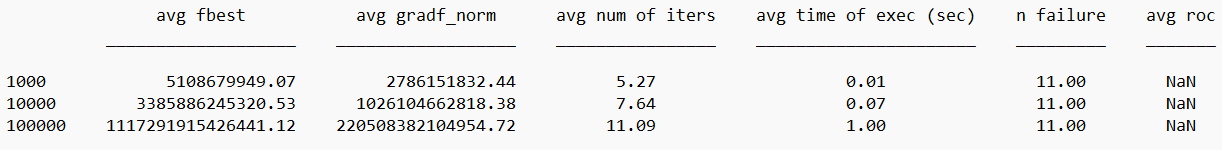
\includegraphics[width=1\textwidth]{img/pb75_table_MN_REL_2.png}
    \caption{Results obtained by running the Modified Newton method on problem 75 using approximated derivatives with $h_i=10^{-2}|\hat{x_i|}$.} 
\end{figure}

\begin{figure}[H]
    \centering
    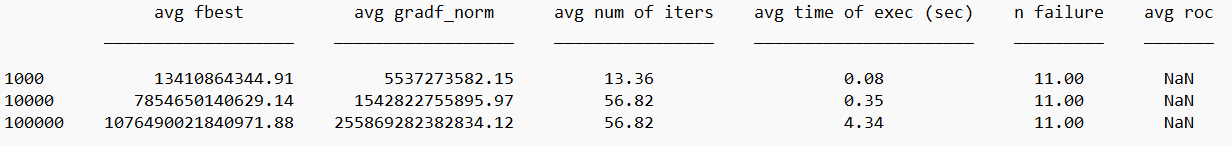
\includegraphics[width=1\textwidth]{img/pb75_table_MN_REL_4.png}
    \caption{Results obtained by running the Modified Newton method on problem 75 using approximated derivatives with $h_i=10^{-4}|\hat{x_i|}$.} 
\end{figure}

\begin{figure}[H]
    \centering
    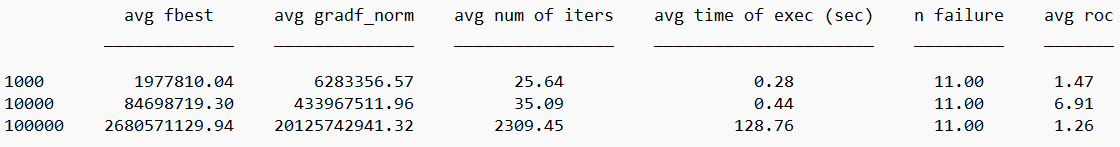
\includegraphics[width=1\textwidth]{img/pb75_table_MN_REL_6.png}
    \caption{Results obtained by running the Modified Newton method on problem 75 using approximated derivatives with $h_i=10^{-6}|\hat{x_i|}$.} 
\end{figure}

\begin{figure}[H]
    \centering
    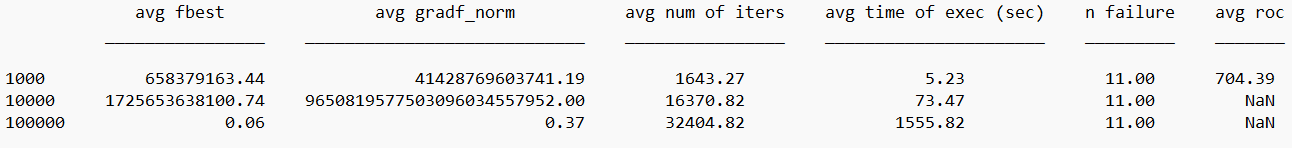
\includegraphics[width=1\textwidth]{img/pb75_table_MN_REL_8.png}
    \caption{Results obtained by running the Modified Newton method on problem 75 using approximated derivatives with $h_i=10^{-8}|\hat{x_i|}$.} 
\end{figure}

\begin{figure}[H]
    \centering
    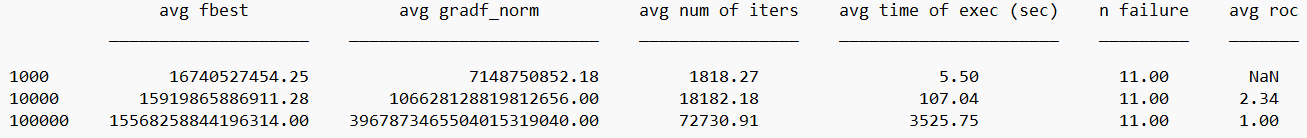
\includegraphics[width=1\textwidth]{img/pb75_table_MN_REL_10.png}
    \caption{Results obtained by running the Modified Newton method on problem 75 using approximated derivatives with $h_i=10^{-10}|\hat{x_i|}$.} 
\end{figure}

\begin{figure}[H]
    \centering
    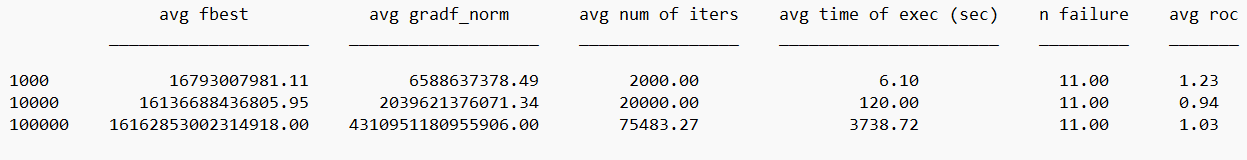
\includegraphics[width=1\textwidth]{img/pb75_table_MN_REL_12.png}
    \caption{Results obtained by running the Modified Newton method on problem 75 using approximated derivatives with $h_i=10^{-12}|\hat{x_i|}$.} 
\end{figure}

The rate of convergence \texttt{NaN} that is sometimes shown is due to failures that occur before having performed the minimum number of iterations 
needed to compute it (which is three since we know the exact value of the solution).

We can identify two different kind of failures that occur: those due to backtracking and those due to the reach of the maximum number of iterations.
In particular, for $h_i=10^{-k}|\hat{x_i}|$ for $k=2,4,6$ all the failures are because of backtracking (they can occur even for smaller $h$, but less frequently). 
This happens because, since $h$ is too large, the approximation 
of the gradient and the Hessian are not good enough to guarantee that a good descent direction is found. For 
all the points, we obtain something similar to the following pathological case:
\begin{list}{}{\setlength{\leftmargin}{0.7cm}}
    \item \texttt{**** REL with h = 1e-06 FOR THE PB 75 (point 8, dimension 10000):  ***** \\
    Time: 0.37252 seconds \\
    Backtracking parameters (rho, c1): 0.8 1e-05 \\
    **** MODIFIED NEWTON METHOD : RESULTS ***** \\
    ************************************ \\
    f(xk): 39458126.9661 \\
    norma di gradf(xk): 414870519.4969 \\
    N. of Iterations: 18/20000 \\
    Rate of Convergence: 8.7683 \\
    ************************************ \\
    FAIL \\
    Failure due to backtracking \\
    cos of the angle between the last computed direction and the gradient: -1.6049e-05 \\
    ************************************
    }
\end{list}
where we can note that after few iterations, becktracking fails because the cosine of the angle between the computed descent direction
and the gradient is so close to zero that this direction is almost perpendicular to the gradient and so tangent to the contour lines of $F$.

The second kind of failure occur for $h_i=10^{-k}|\hat{x_i}|$ for $k=8, 10, 12$. The best results are obtained with $k=8$, because, with most starting points, 
when the method reaches the maximum number of iterations allowed, the current solution is quite close to zero. One example is the following:
\begin{list}{}{\setlength{\leftmargin}{0.7cm}}
    \item \texttt{**** REL with h = 1e-08 FOR THE PB 75 (point 10, dimension 100000):  *****\\
    Time: 4376.7099 seconds\\
    Backtracking parameters (rho, c1): 0.8 1e-05\\
    **** MODIFIED NEWTON METHOD : RESULTS *****\\
    ************************************\\
    f(xk): 0.0060851\\
    norma di gradf(xk): 0.0012706\\
    N. of Iterations: 80000/80000\\
    Rate of Convergence: 0.058907\\
    ************************************\\
    FAIL\\
    Failure not due to backtracking\\
    ************************************\\
    }
\end{list}
Still, the behaviour is very irregular and we can see it for example from the experimental rate of convergence, which is completely
different from the theoretical one.

For $k=10, 12$ we have very poor results: the method fails in most cases because of the maximum number of iterations, but the solution found 
is very far from the exact one. This is due to numerical cancellation that occurs when computing the approximations of 
the derivatives since we are subtracting two numbers very close to each other. So the approximations obtained are completely inaccurate and cause
the method to perform this poorly. One example is the following:
\begin{list}{}{\setlength{\leftmargin}{0.7cm}}
    \item \texttt{**** REL with h = 1e-12 FOR THE PB 75 (point 8, dimension 100000):  ***** \\
    Time: 3679.4492 seconds\\
    Backtracking parameters (rho, c1): 0.8 1e-05\\
    **** MODIFIED NEWTON METHOD : RESULTS *****\\
    ************************************\\
    f(xk): 1.756805324787388e+16\\
    norma di gradf(xk): 698990881722798.6\\
    N. of Iterations: 80000/80000\\
    Rate of Convergence: 0.86925\\
    ************************************\\
    FAIL\\
    Failure not due to backtracking\\
    ************************************\\
    }
\end{list}

When constant values of $h$ are used, the behaviour is similar: for $h=10^{-k}$, $k=2,4,6$ we always have failures due to backtracking and 
for $h=10^{-k}$, $k=10,12$ most failures occur because of the reach of the maximum number of iterations, producing a solution very far from the exact one.

For $h=10^{-8}$ the behaviour is again the best, with no failures occurring for dimension $n=10^3$ and $n=10^4$ and some failures due to backtracking 
for $n=10^5$, but happening when the method is close to the exact solution. We report here two examples of this:
\begin{list}{}{\setlength{\leftmargin}{0.7cm}}
    \item \texttt{**** COST with h = 1e-08 FOR THE PB 75 (point 1, dimension 1000):  *****\\
    Time: 4.7991 seconds\\
    Backtracking parameters (rho, c1): 0.8 1e-05\\
    **** MODIFIED NEWTON METHOD : RESULTS *****\\
    ************************************\\
    f(xk): 1.361e-05\\
    norma di gradf(xk): 9.9781e-05\\
    N. of Iterations: 1699/2000\\
    Rate of Convergence: 0.9956\\
    ************************************\\
    SUCCESS\\
    ************************************\\
    } 
\end{list}
\begin{list}{}{\setlength{\leftmargin}{0.7cm}}
    \item \texttt{**** COST with h = 1e-08 FOR THE PB 75 (point 11, dimension 100000):  *****\\
    Time: 155.1714 seconds\\
    Backtracking parameters (rho, c1): 0.8 1e-05\\
    **** MODIFIED NEWTON METHOD : RESULTS *****\\
    ************************************\\
    f(xk): 0.012298\\
    norma di gradf(xk): 0.32072\\
    N. of Iterations: 4748/80000\\
    Rate of Convergence: 1.5507\\
    ************************************\\
    FAIL\\
    Failure due to backtracking\\
    cos of the angle between last computed direction and the gradient: -0.00022156\\
    ************************************}
\end{list}
